\chapter{Experimental Results}
This chapter will cover the multiple experiments conducted, it will cover a comparison of Boltzmann exploration and epsilon greedy exploration and experiments with different hyperparameters and how this affects the results.

\section{CartPole Outcomes}
The first task developed was the classic CartPole environment,
this was helpful in understanding core concepts of reinforcement learning and neural networks, along with it,
CartPole was essential in testing and setting up the logging interface as well as testing different implementations of the learning algorithm 
\subsection*{Keras-rl}
Keras-rl is a community maintained high-level implementation of Keras agents for reinforcement learning. 
this was the first implementation tested.
%%%%%%%%% INSERT DETAILS HERE %%%%%%%%%

The implementation of Keras-rl is very easy and doesn't require a deep understanding of reinforcement learning and the learning structures.
\subsection*{Keras API}
The second implementation tested was using the plain Keras API. While this provides more flexibility, it also requires a much deeper understanding of how reinforcement learning works.
%%%%%%%%% INSERT DETAILS HERE %%%%%%%%%
The implementation using the Keras API was essential to develop the necessary knowledge for the project and to progress to the next stage.

While an implementation using Keras-rl would be simpler and even possibly ease the iteration process, this implementation provides less flexibility and given the target of the project and 
desire to develop a deeper understanding of reinforcement learning, the implementation using the Keras API was chosen to implement the next phases.

\subsection*{Results}
The CartPole served as an initial testing environment for multiple variables and strategies.

The first attempt uses Boltzmann distribution as an exploration policy %try to explain what Boltzmann is%
in this experiment, an iteration on the learning rate was performed, along with the number of steps to achieve the target.

\begin{figure}[H]
 \centering
 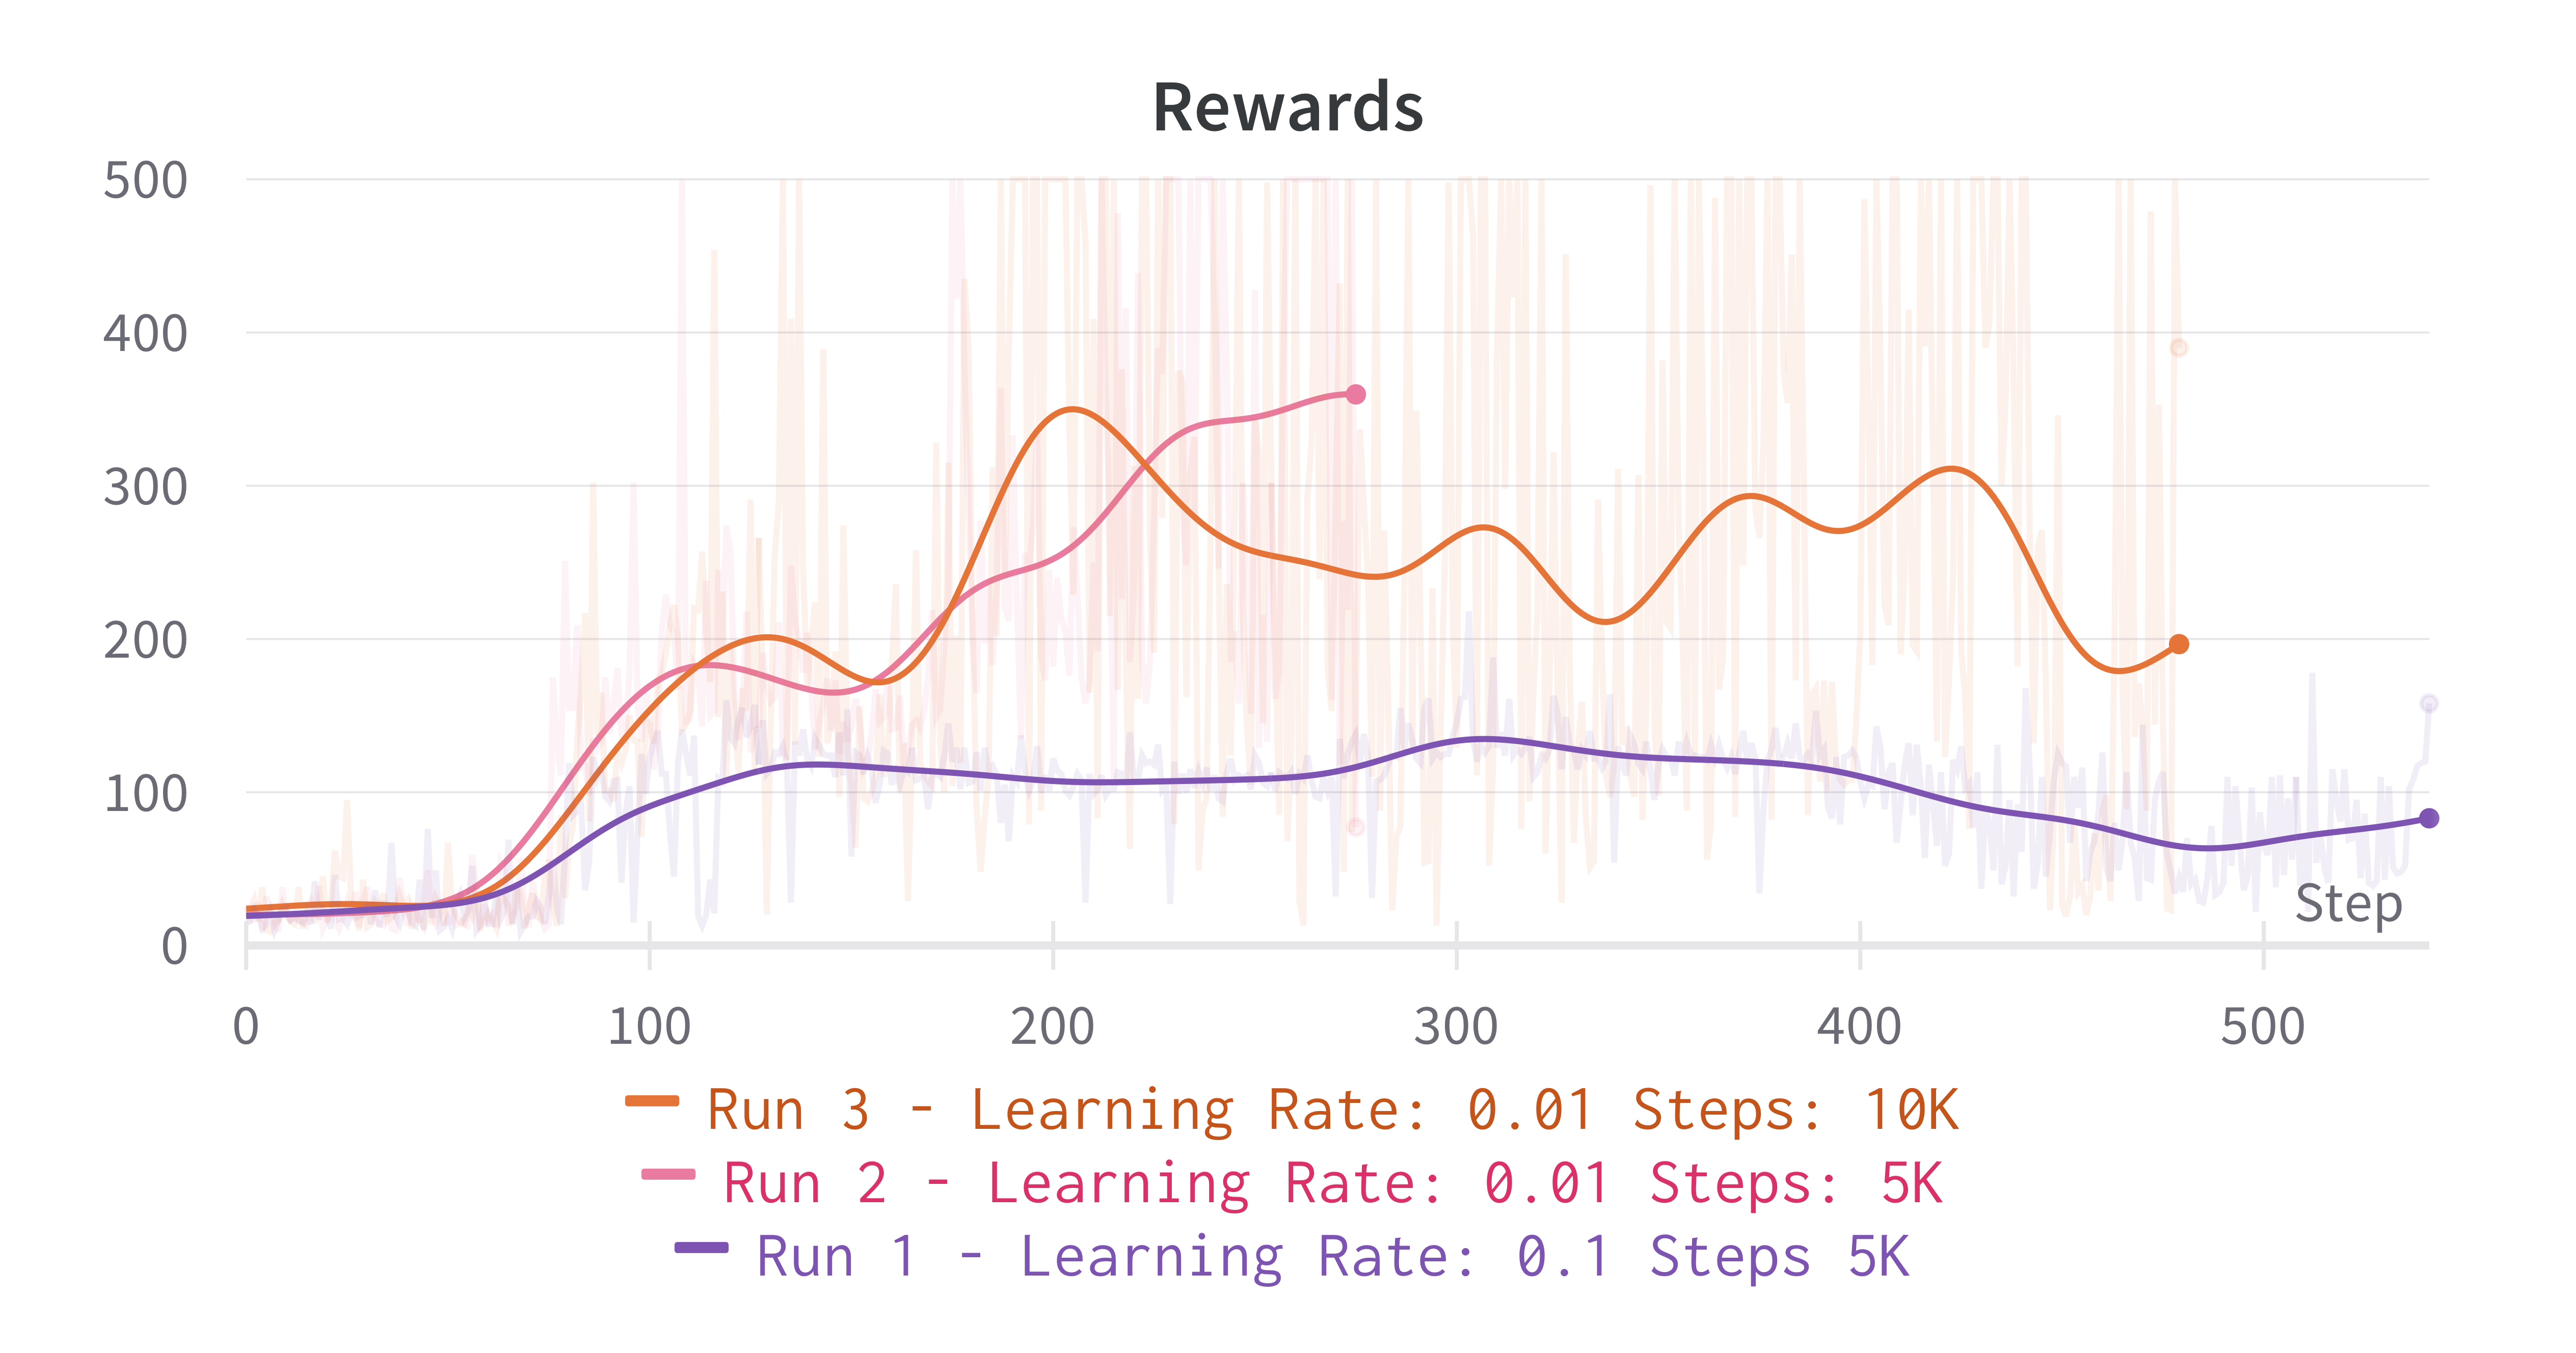
\includegraphics[width=1\textwidth]{charts/rewards_cartpole.png}
 \caption{Reward output for the CartPole experiment - Boltzmann. }
 \end{figure}

% \begin{figure}[H]
% \centering
% 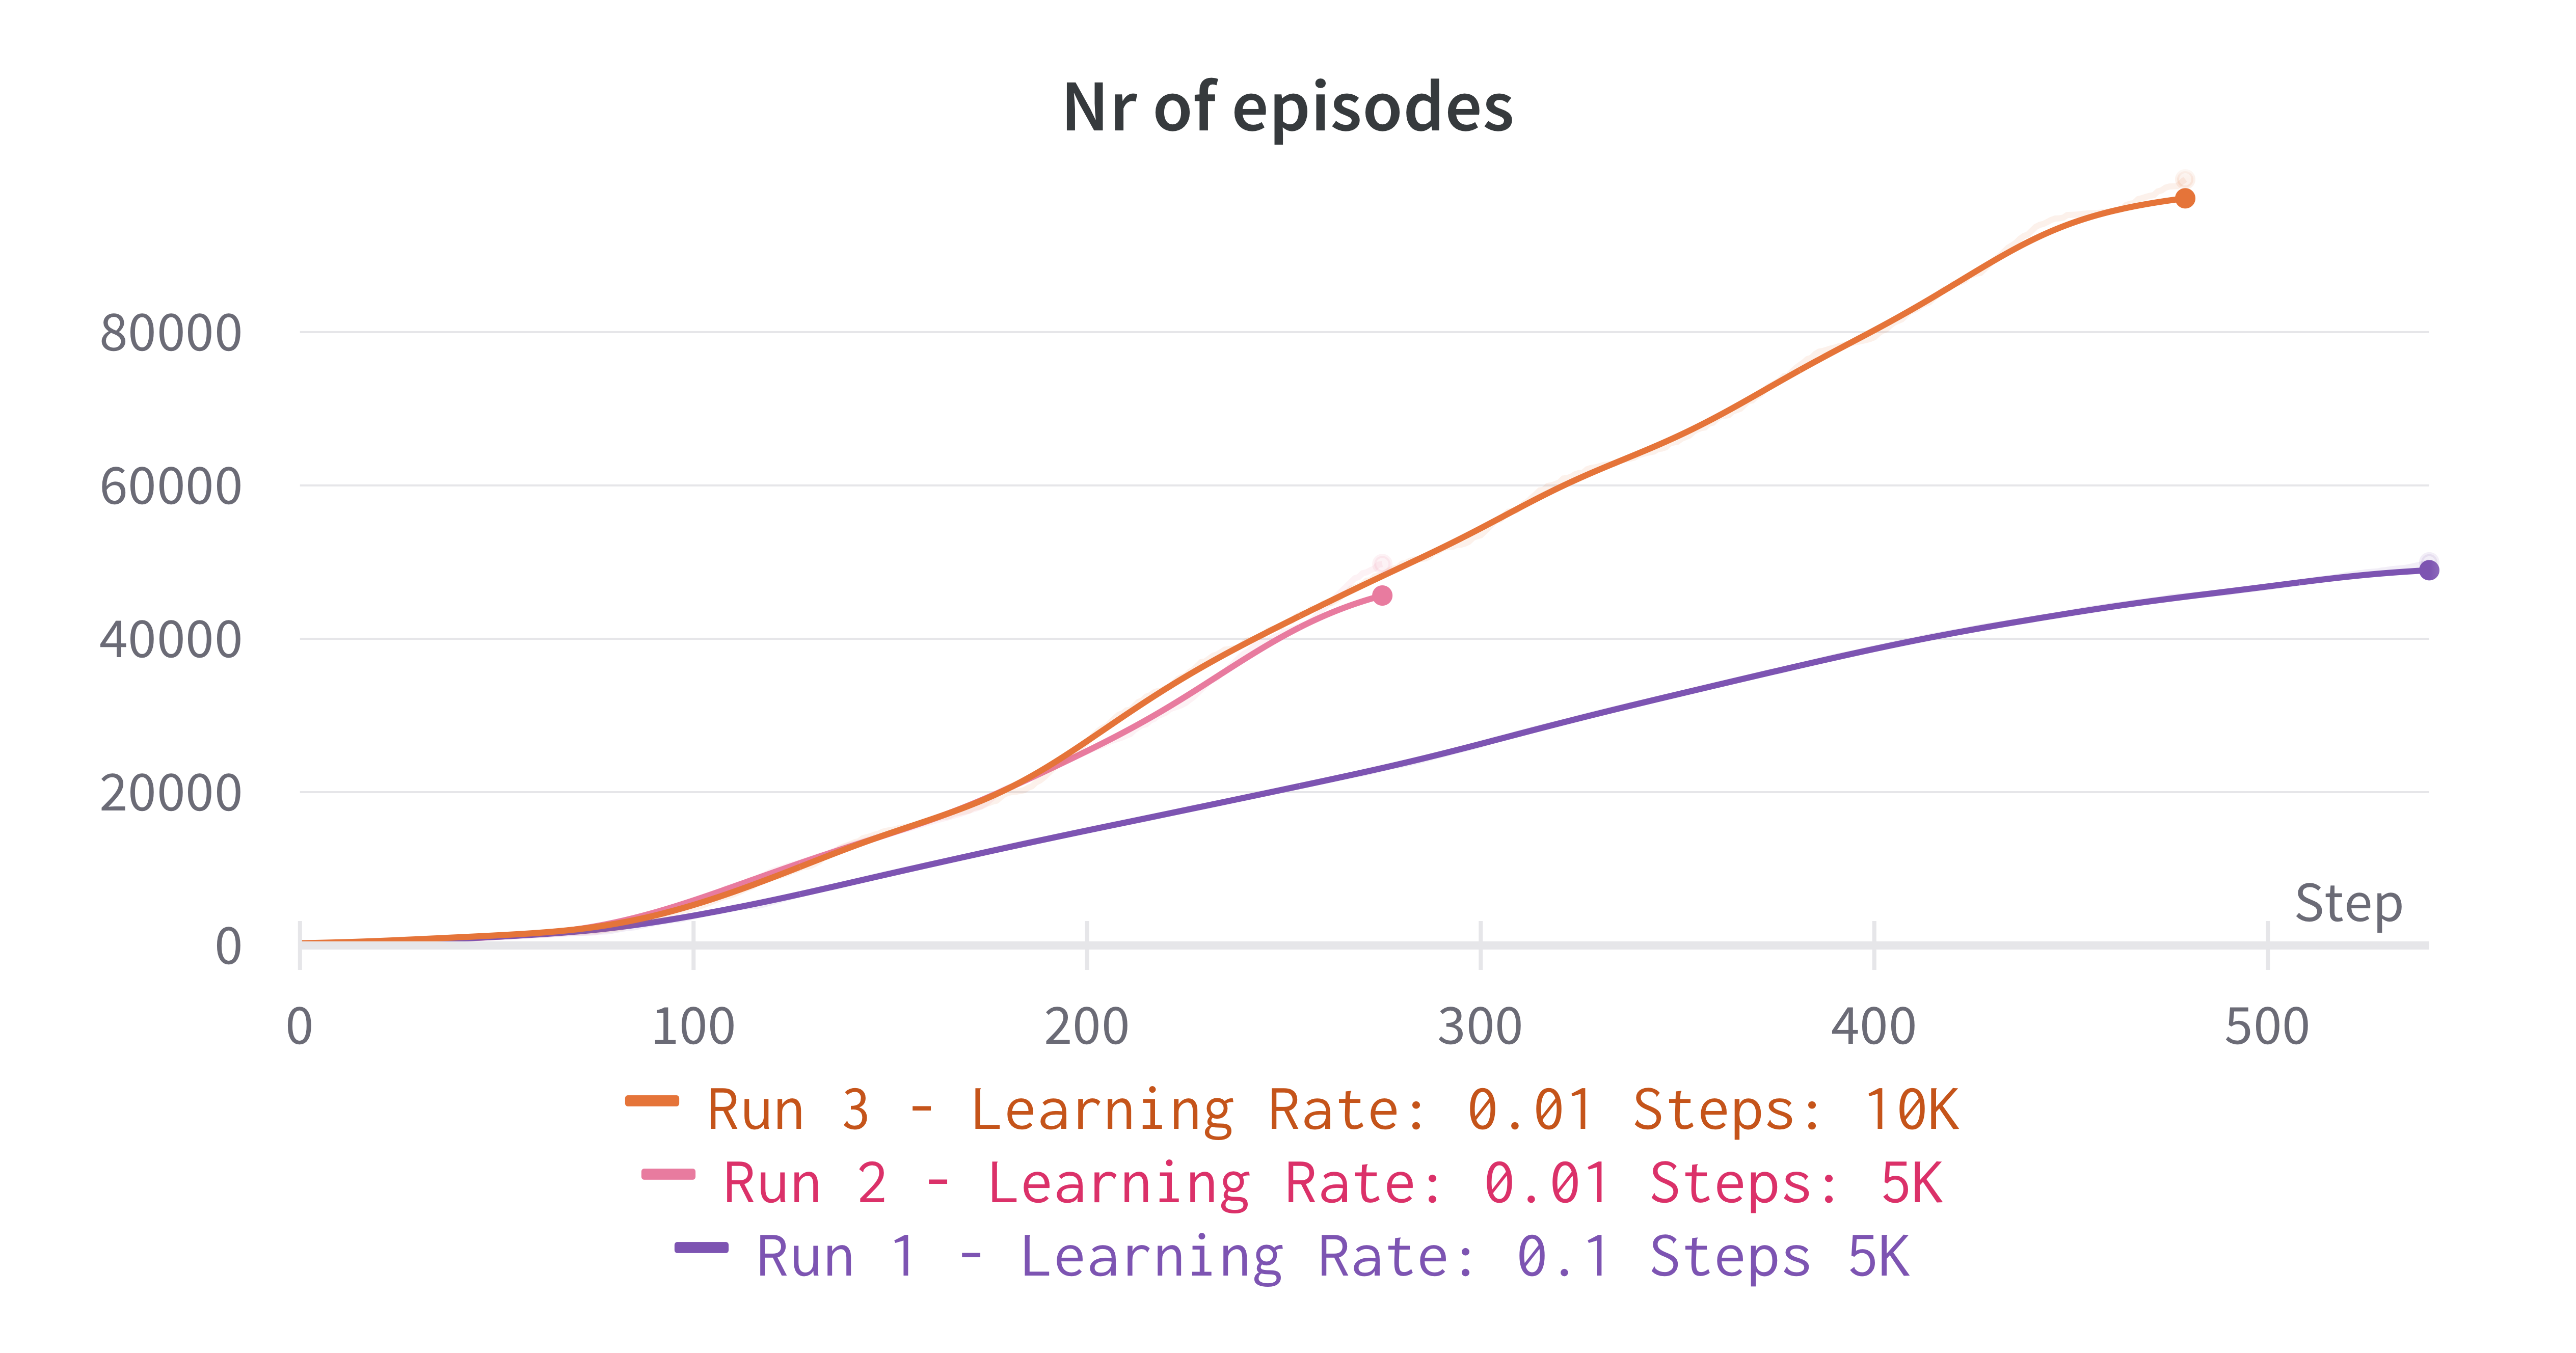
\includegraphics[width=1\textwidth]{charts/episodes_cartpole.png}
% \caption{Number of episodes for the CartPole experiment}
% \end{figure}
As can be seen from the above graphs, the learning rate of 0.01 shows much better results when compared to 0.1, although when the model was tested after 5000 steps, the results were as follows:
\begin{table}[H]
 \caption{20 test runs for the CartPole experiment, comparing the results of two different training lengths.}

 \begin{tabular}{ |p{2.2cm}|p{3cm}|p{3cm}| }
 \cline{2-3} 
 \multicolumn{1}{c}{} & \multicolumn{2}{|c|}{ \textbf{20 episodes test run}} \\
 \cline{2-3} 
 \multicolumn{1}{c}{} & \multicolumn{1}{|c|}{Learning Rate: 0.01} & \multicolumn{1}{|c|}{Learning Rate: 0.01}\\
 \multicolumn{1}{c}{} & \multicolumn{1}{|c|}{Steps 5000} & \multicolumn{1}{|c|}{Steps: 10000}\\
 \hline
 Episode 1 & 126.00 & 500.00\\
 Episode 2 & 121.00 & 500.00\\
 Episode 3 & 129.00 & 500.00\\
 Episode 4 & 124.00 & 500.00\\
 Episode 5 & 124.00 & 500.00\\
 Episode 6 & 123.00 & 500.00\\
 Episode 7 & 122.00 & 500.00\\
 Episode 8 & 123.00 & 500.00\\
 Episode 9 & 124.00 & 500.00\\
 Episode 10 & 123.00 &500.00 \\
 Episode 11 & 125.00 &500.00 \\
 Episode 12 & 116.00 &500.00 \\
 Episode 13 & 125.00 &500.00 \\
 Episode 14 & 126.00 &500.00 \\
 Episode 15 & 125.00 &500.00 \\
 Episode 16 & 127.00 &500.00 \\
 Episode 17 & 118.00 &500.00 \\
 Episode 18 & 125.00 &500.00 \\
 Episode 19 & 122.00 &500.00 \\
 Episode 20 & 119.00 &500.00 \\
 \hline
 \multicolumn{1}{c}{} & \multicolumn{1}{|c|}{\textbf{Average: 123.35}} & \multicolumn{1}{|c|}{\textbf{Average: 500.00}} \\
 \cline{2-3}
 \multicolumn{3}{c}{} 
 \end{tabular}
\end{table}
 
 As we can observe from the table, the training length can have a significant impact on the results, 
 in the case of the CartPole environment, it helps to break harmful correlations, stopping the cart from moving of the boundaries. 

 The second attempt uses a more common exploration policy, epsilon greedy, in this experiment the $\epsilon$, learning rate and metric used were also varied.
 \begin{figure}[H]
 \centering
 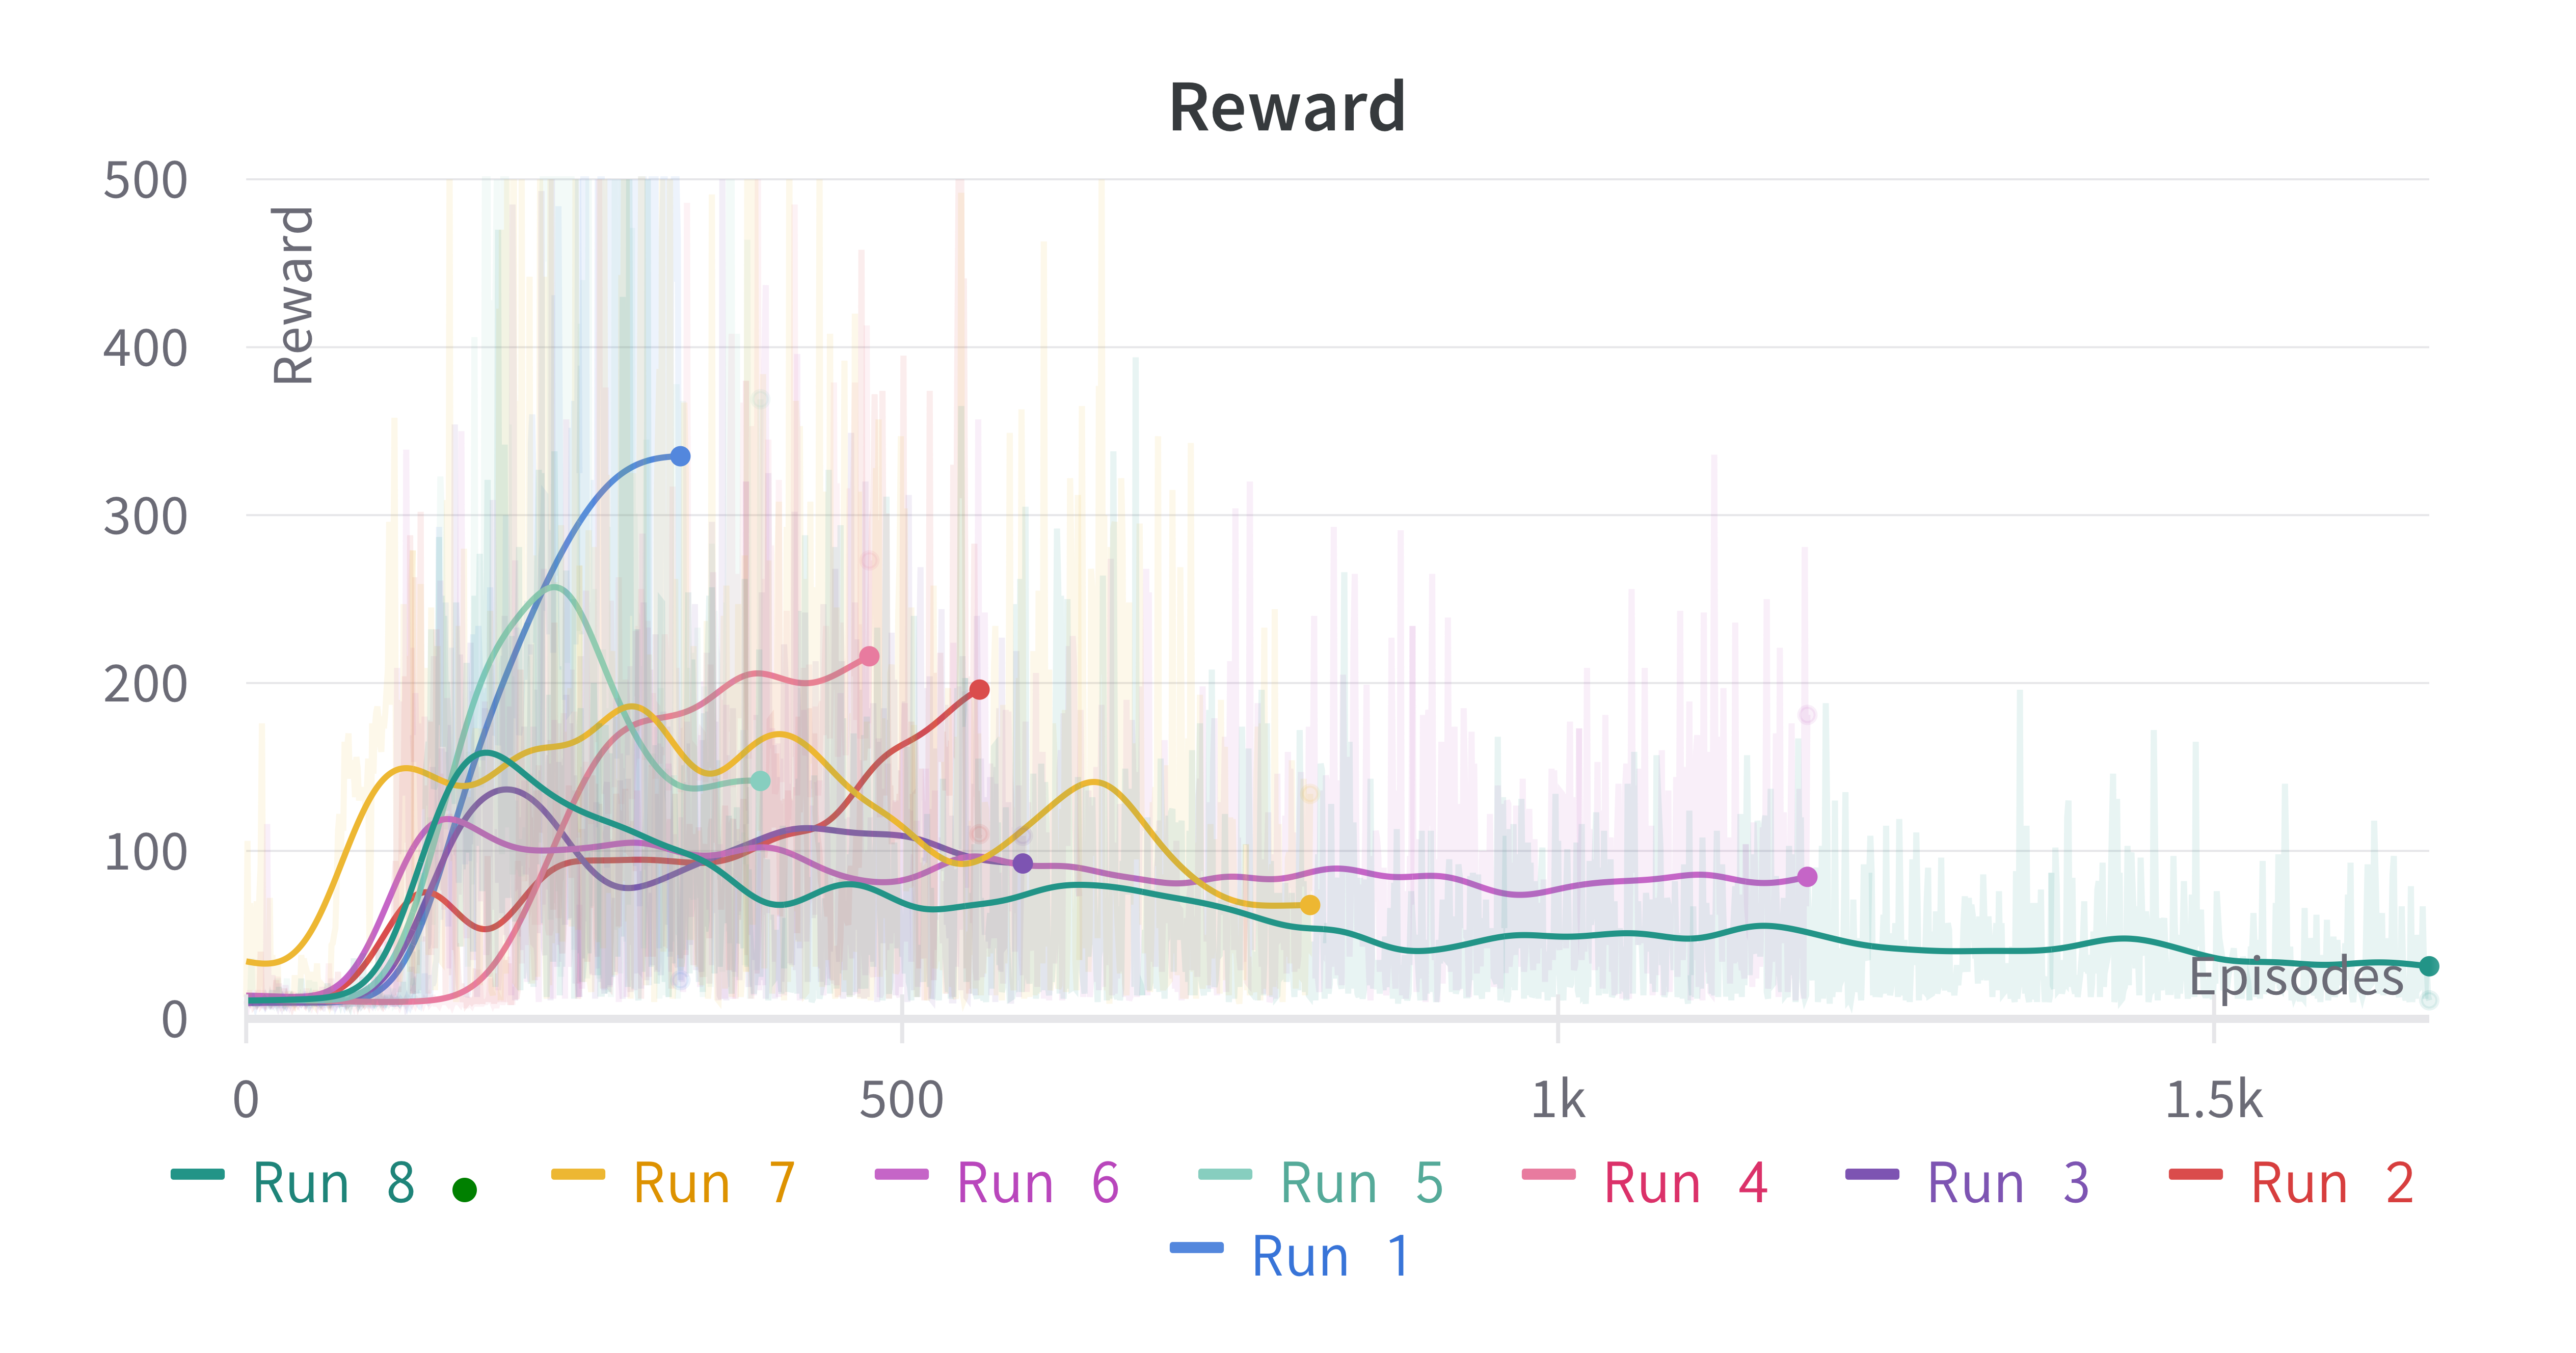
\includegraphics[width=1\textwidth]{charts/eps_greedy.png}
 \caption{Reward output for the CartPole experiment - epsilon greedy.}
 \end{figure}
 
\begin{center}
 \begin{table}[H]
 \caption{Hyperparameters for each of the 8 runs using epsilon greedy.}

 \begin{tabular}{|l|l|l|l|l|l|l|l|l|}
 \hline
 Hyperparameters & Run 1 & Run 2 & Run 3 & Run 4 & Run 5 & Run 6 & Run 7 & Run 8 \\ \hline
 epsilon & 0.1 & 0.1 & 0.1 & 0.1 & 0.1 & 0.1 & 0.2 & 0.3 \\ \hline
 learning rate & 0.01 & 0.1 & 0.03 & 0.001 & 0.01 & 0.03 & 0.01 & 0.01 \\ \hline
 metric & mae & mae & mae & mae & accuracy & mae & mae & mae \\ \hline
 number of steps & 50000 & 50000 & 50000 & 50000 & 50000 & 100000 & 100000& 100000 \\ \hline
 \end{tabular}
 \end{table}
\end{center}
 
 \begin{table}[H]
 \caption{Results for 20 test episodes for each of the eight training sessions. In the tests, all actions are chosen using the trained model.}

 \begin{tabular}{l|l|l|l|l|l|l|l|l|}
 \cline{2-9}
 & Run 1 & Run 2 & Run 3 & Run 4 & Run 5 & Run 6& Run 7 & Run 8 \\ \hline
 \multicolumn{1}{|l|}{Episode 1} & 500.00 & 31.00 & 47.00 & 390.00 & 500.00 & 88.00& 500.00 & 89.00\\
 \multicolumn{1}{|l|}{Episode 2} & 500.00 & 28.00 & 49.00 & 338.00 & 500.00 & 87.00& 500.00 & 95.00\\
 \multicolumn{1}{|l|}{Episode 3} & 500.00 & 85.00 & 33.00 & 500.00 & 500.00 & 84.00& 500.00 & 90.00\\
 \multicolumn{1}{|l|}{Episode 4} & 500.00 & 85.00 & 26.00 & 166.00 & 500.00 & 90.00& 500.00 & 92.00\\
 \multicolumn{1}{|l|}{Episode 5} & 500.00 & 28.00 & 51.00 & 210.00 & 500.00 & 91.00& 500.00 & 88.00\\
 \multicolumn{1}{|l|}{Episode 6} & 500.00 & 28.00 & 57.00 & 307.00 & 500.00 & 88.00& 500.00 & 93.00\\
 \multicolumn{1}{|l|}{Episode 7} & 500.00 & 34.00 & 41.00 & 335.00 & 500.00 & 86.00& 500.00 & 95.00\\
 \multicolumn{1}{|l|}{Episode 8} & 500.00 & 27.00 & 22.00 & 343.00 & 500.00 & 91.00& 500.00 & 92.00\\
 \multicolumn{1}{|l|}{Episode 9} & 500.00 & 85.00 & 80.00 & 307.00 & 500.00 & 86.00& 500.00 & 87.00\\
 \multicolumn{1}{|l|}{Episode 10} & 500.00 & 33.00 & 21.00 & 500.00 & 500.00 & 92.00& 500.00 & 92.00\\
 \multicolumn{1}{|l|}{Episode 11} & 500.00 & 28.00 & 26.00 & 139.00 & 500.00 & 29.00& 500.00 & 90.00\\
 \multicolumn{1}{|l|}{Episode 12} & 500.00 & 83.00 & 90.00 & 437.00 & 500.00 & 87.00& 500.00 & 87.00\\
 \multicolumn{1}{|l|}{Episode 13} & 500.00 & 30.00 & 75.00 & 341.00 & 500.00 & 90.00& 500.00 & 91.00\\
 \multicolumn{1}{|l|}{Episode 14} & 500.00 & 33.00 & 56.00 & 500.00 & 500.00 & 88.00& 500.00 & 90.00\\
 \multicolumn{1}{|l|}{Episode 15} & 500.00 & 88.00 & 41.00 & 493.00 & 500.00 & 87.00& 500.00 & 93.00\\
 \multicolumn{1}{|l|}{Episode 16} & 500.00 & 31.00 & 88.00 & 500.00 & 500.00 & 86.00& 500.00 & 91.00\\
 \multicolumn{1}{|l|}{Episode 17} & 500.00 & 29.00 & 39.00 & 500.00 & 500.00 & 81.00& 500.00 & 93.00\\
 \multicolumn{1}{|l|}{Episode 18} & 500.00 & 35.00 & 33.00 & 500.00 & 500.00 & 87.00& 500.00 & 89.00\\
 \multicolumn{1}{|l|}{Episode 19} & 500.00 & 83.00 & 67.00 & 340.00 & 500.00 & 94.00& 500.00 & 93.00\\
 \multicolumn{1}{|l|}{Episode 20} & 500.00 & 32.00 & 77.00 & 242.00 & 500.00 & 87.00& 500.00 & 92.00\\ \hline
 \multicolumn{1}{|l|}{\textbf{Average}} & 500.00 & 46.80 & 50.95 & 369.40 & 500.00 & 84.95 & 500.00 &91.10 \\
 \hline
 \end{tabular}
 \end{table}

 When comparing the two approaches(epsilon greedy and Boltzmann), it is clear that the more common epsilon greedy approach was more successful in solving the CartPole environment, achieving the maximum of 500 points in 50000 steps.

 As can be observed by the table containing the average reward for 20 test episodes, we can observe that both run 1 and run 5 were successful with 50000 steps, followed by run 4 with close scores.
 Both run 1 and 5 have 0.01 as the learning rate and only vary the metric used, any learning rate above 0.01 tested yielded low scores, when testing varying epsilons it was possible to solve the environment with double the steps, 
 the results also demonstrate that setting random exploration to values higher than 20\% couldn't be solved under the 10000 steps.

 The conclusion drawn show that the most suitable parameters are:
 \begin{itemize}
 \item \textbf{epsilon} = 0.1
 \item \textbf{learning rate} = 0.01
 \item \textbf{metric} = mae
 \item \textbf{number of steps} = 50000
 \end{itemize}
 
 \section{2D Environment Outcomes}
%%%%%%% MIGHT NOT BELONG HERE %%%%%%%%%%
When first implementing the 2D environment using the Keras-rl library, it was found that the library doesn't support the use of Multidiscrete action spaces, 
an attempt to implement this environment using TensorFlow Agents yielded the same results by only supporting scalar actions.

Given this, it was necessary to implement a custom learning implementation using the Keras API.
%%%%%%% MIGHT NOT BELONG HERE %%%%%%%%%%

The 2D environment was a big challenge to develop, this is due to the big jump in complexity in comparison with a simple, well known and documented environment such as the CartPole.
The 2D environment required a custom 2D environment, and the implementation of this with the physics engine. When this obstacle was overcome, the second major challenge was to implement the learning algorithm
and be able to control the eight joints simultaneously.

Once the learning algorithm was fully implemented, the reward system and hyperparameters needed to be tested and tuned, this shows the complexity of reinforcement learning. While many iterations over the reward system and hyperparameters were made, given the limited time and resources, a full walking motion could not have been achieved.
Although, the results obtained with experientation were helpfull in understading the impact of the changes in the reward system.
\subsection*{Results}
\begin{figure}[H]
 \centering
 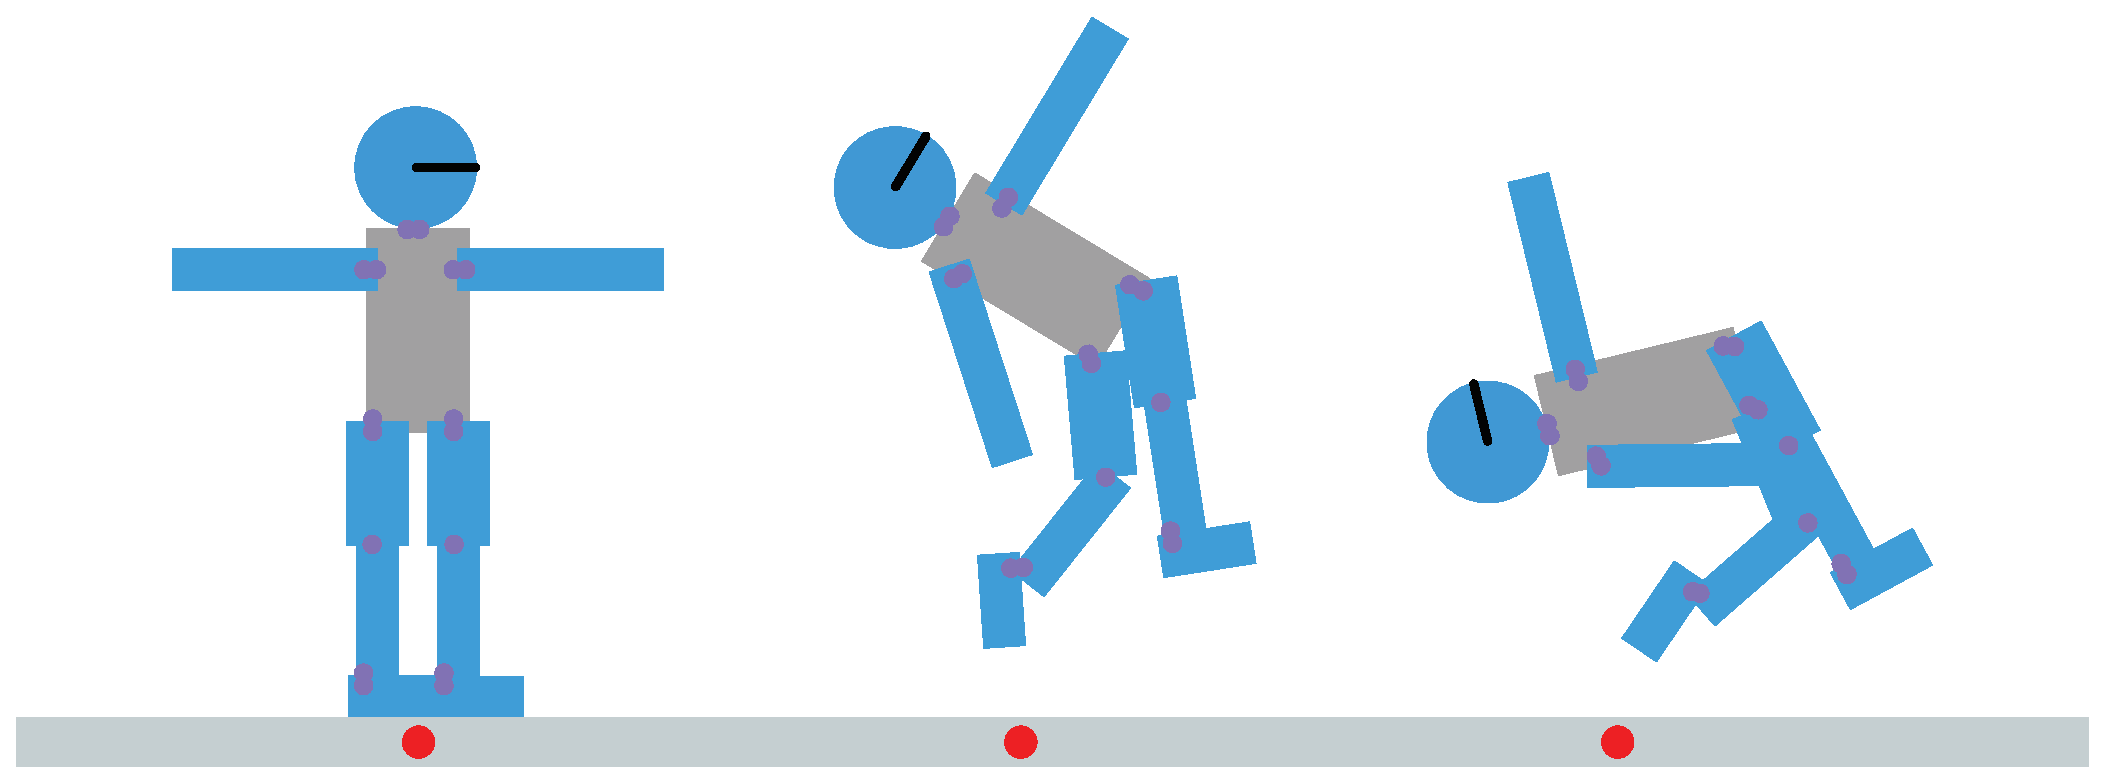
\includegraphics[scale=0.3]{2d_walk_199_episodes}
 \caption{Simulation of 2D environment after 199 episodes, the red dot is a reference used to understand the relative movement of the robot to a stationary point. See text for more details.}
\end{figure}
\begin{figure}[H]
 \centering
 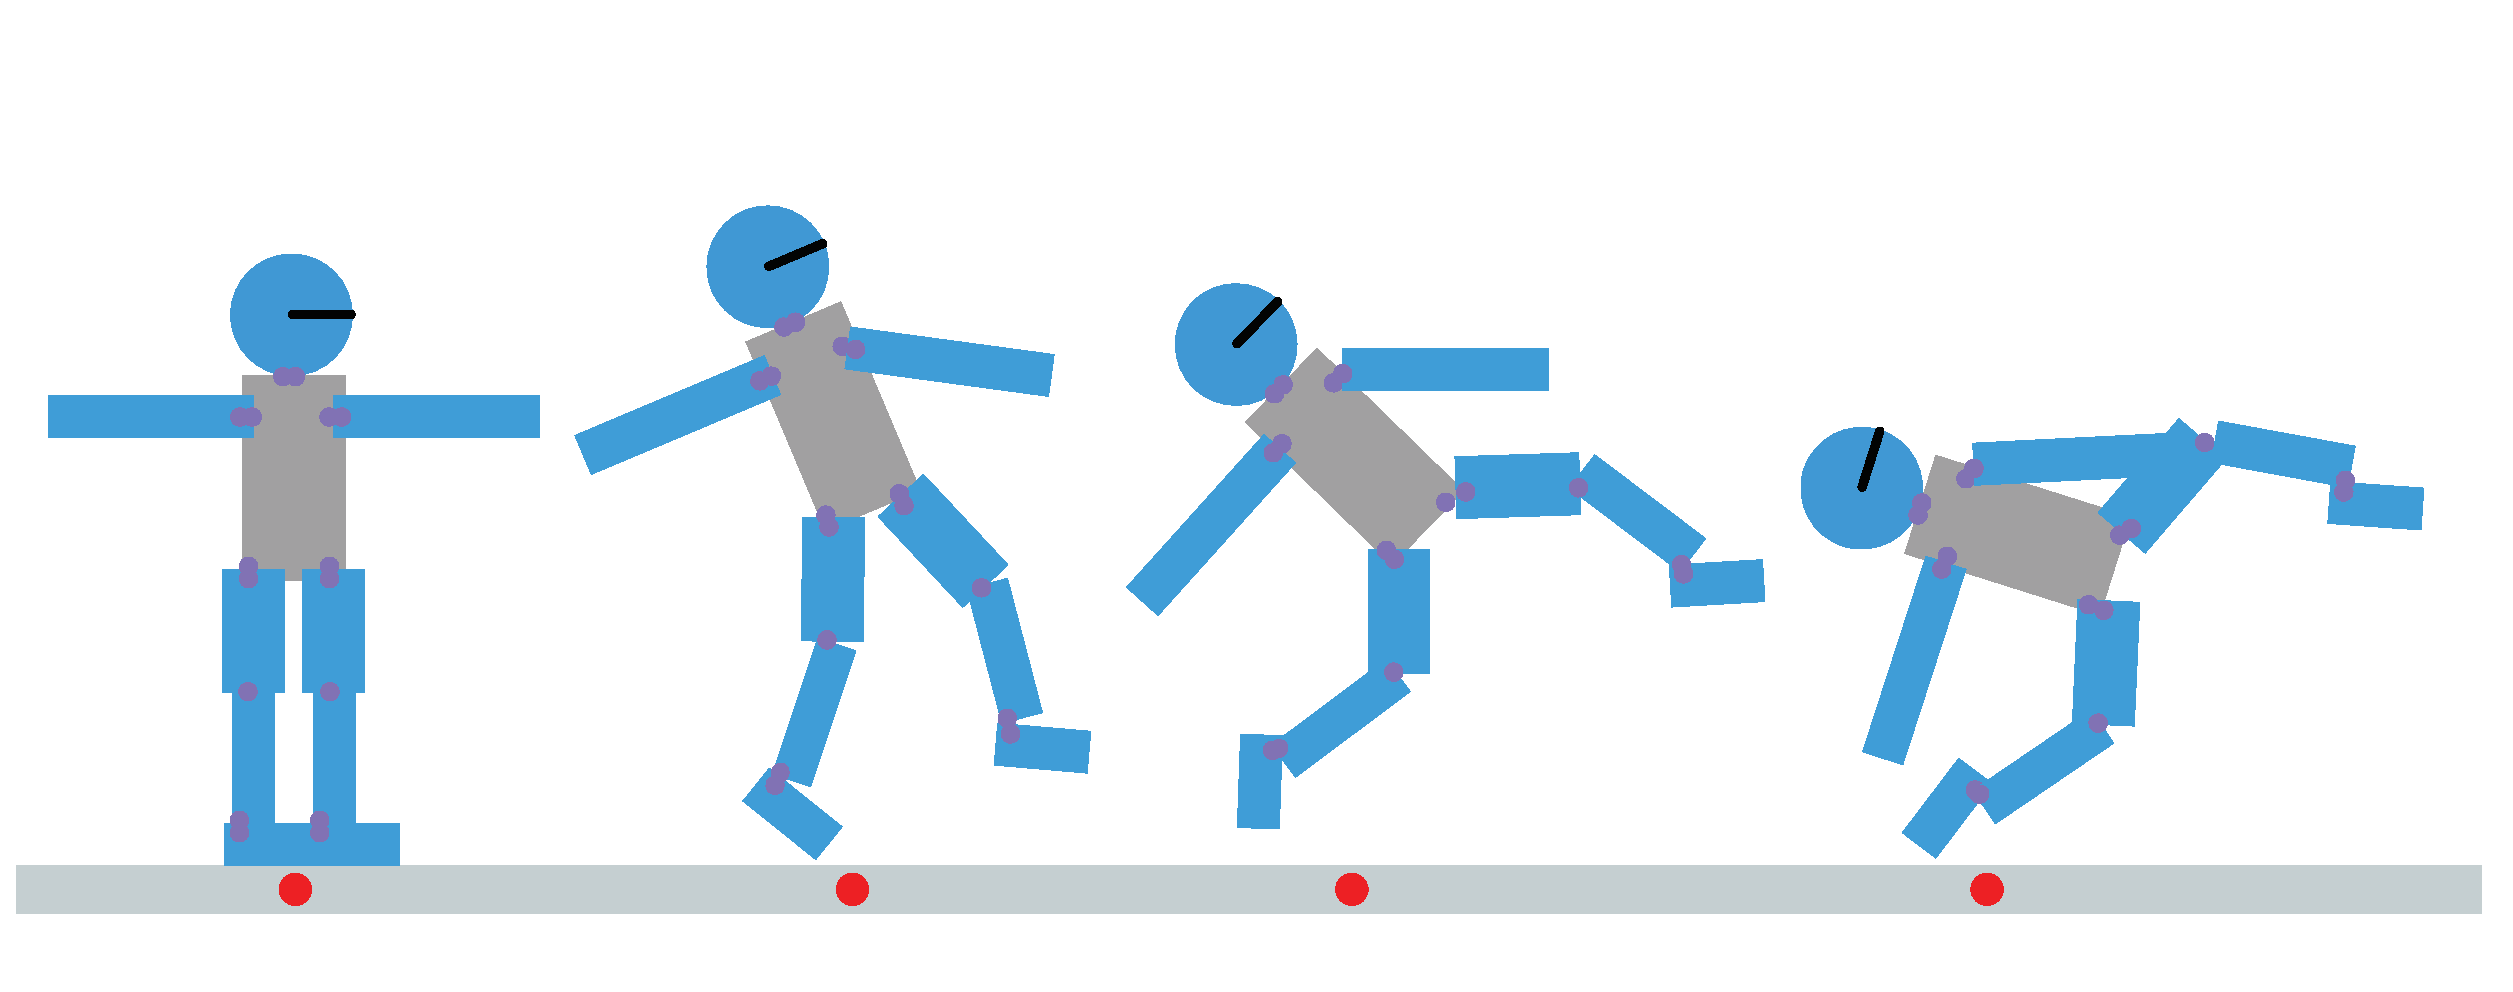
\includegraphics[scale=0.3]{2d_walk_10651_episodes}
 \caption{Simulation of 2D environment after 10651 episodes, the red dot is a reference used to understand the relative movement of the robot to a stationary point. See text for more details.}
\end{figure}

\begin{table}[H]
 \centering
 \caption{hyperparameters from the run demonstrated above.}
 \begin{tabular}{|ll|}
 \hline
 \multicolumn{2}{|c|}{Hyperparameters} \\ \hline
 \multicolumn{1}{|l|}{gamma} & 0.99 \\ \hline
 \multicolumn{1}{|l|}{learning rate} & 0.01 \\ \hline
 \multicolumn{1}{|l|}{epsilon maximum} & 0.1 \\ \hline
 \multicolumn{1}{|l|}{epsilon minimum} & 0.01 \\ \hline
 \multicolumn{1}{|l|}{batch size} & 64 \\ \hline
 \multicolumn{1}{|l|}{units per hidden layer} & 128 \\ \hline
 \multicolumn{1}{|l|}{loss function} & mean absolute error \\ \hline
 \end{tabular}
\end{table}
After 10000 episodes, we start to observe how the agent starts to learn to move forward as it yields the most rewards as opposed to the example of 199 episodes where the agent would jump and fall almost in the starting position.

After many iterations over the reward system and hyperparameters, the reward system performs better when the range of reward is positive. After removing penalties and setting the rewards in the range [0,16], the agent showed more expectable results and was able to learn to reach targets in close range.

One of the observations made during trained is how the agent rapidly learns to balance itself in the same position. This happens because in the short term, it's more favourable to stay still than to fall. This behaviour develops very fast, although, as learning to walk is a complex pattern, it would require long training sessions with potentially millions of episodes to update the neural network.

When testing why the robot wasn't able to learn to walk, the q-values showed very little variation, independently of the input. The reason for this is that the learning rate, when set to 0.01, would require much lengthier training sessions. When applying the same testing to sessions with learning rates as high as 0.1, the q-values would converge very fast, but the agent wouldn't perform well.

Bellow are the comparison of selected runs to which were applied different hyperparameters, as an attempt to find the most suitable and how varying this affects the results.
\begin{figure}[H]
 \centering
 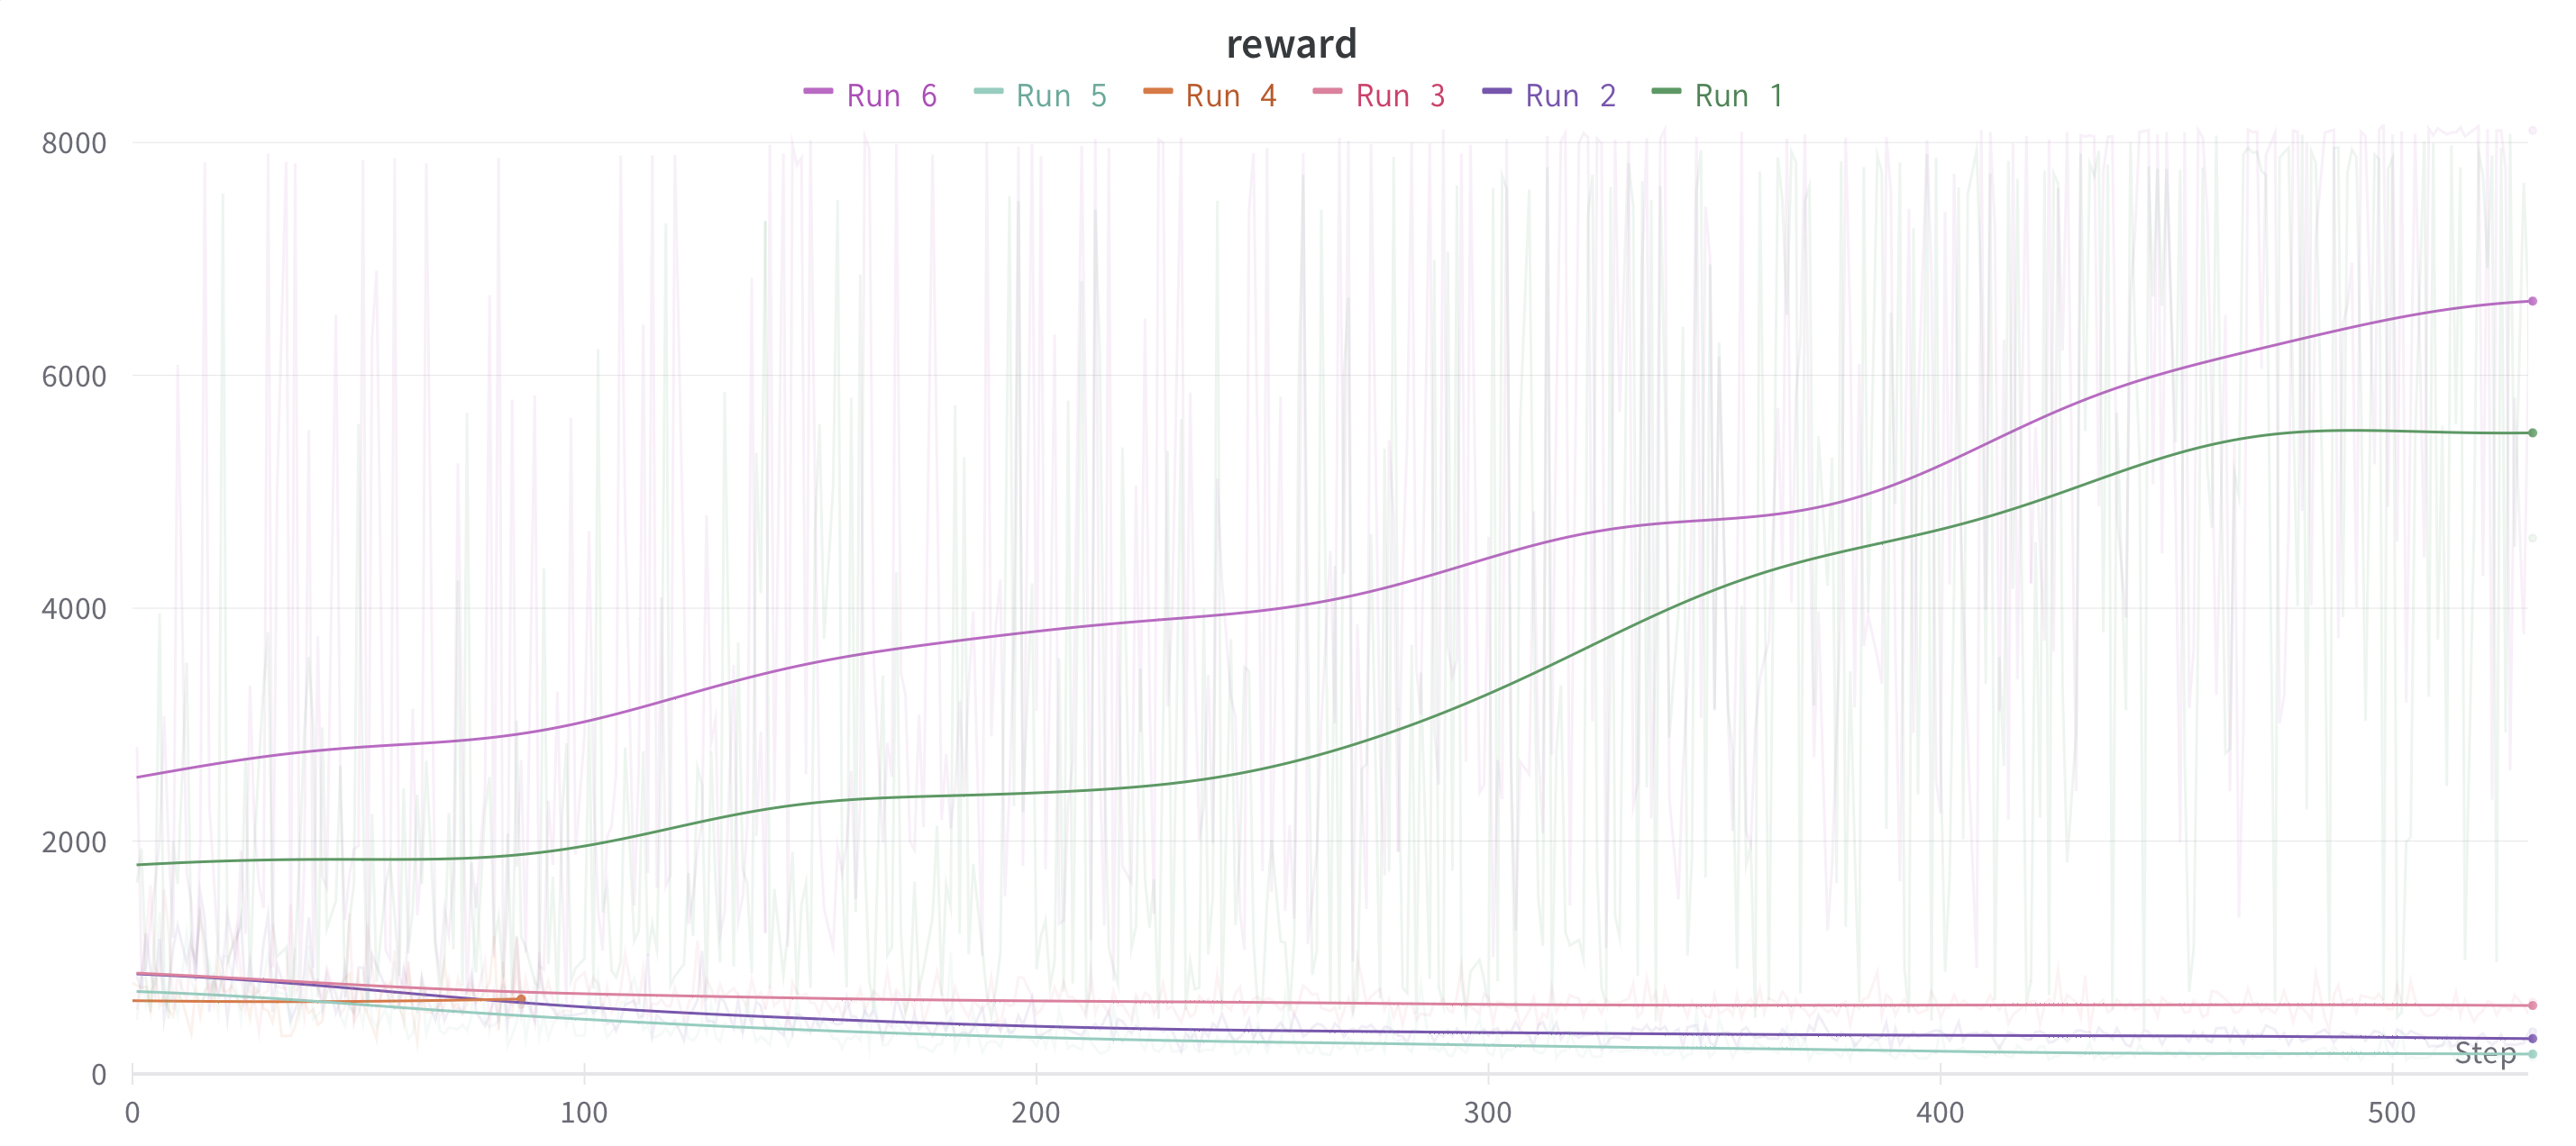
\includegraphics[width=1\textwidth]{select_walker_graph.png}
 \caption{Comparison of multiple selected runs using different hyperparameters. See table \ref*{table:graph_walker} for hyperparameters}
\end{figure}

From the graph above we can observe that two of the runs perform much better than the remaining, this is explained, confirming previous beliefs, by using an importance and correlation analysis:
\begin{figure}[H]
 \centering
 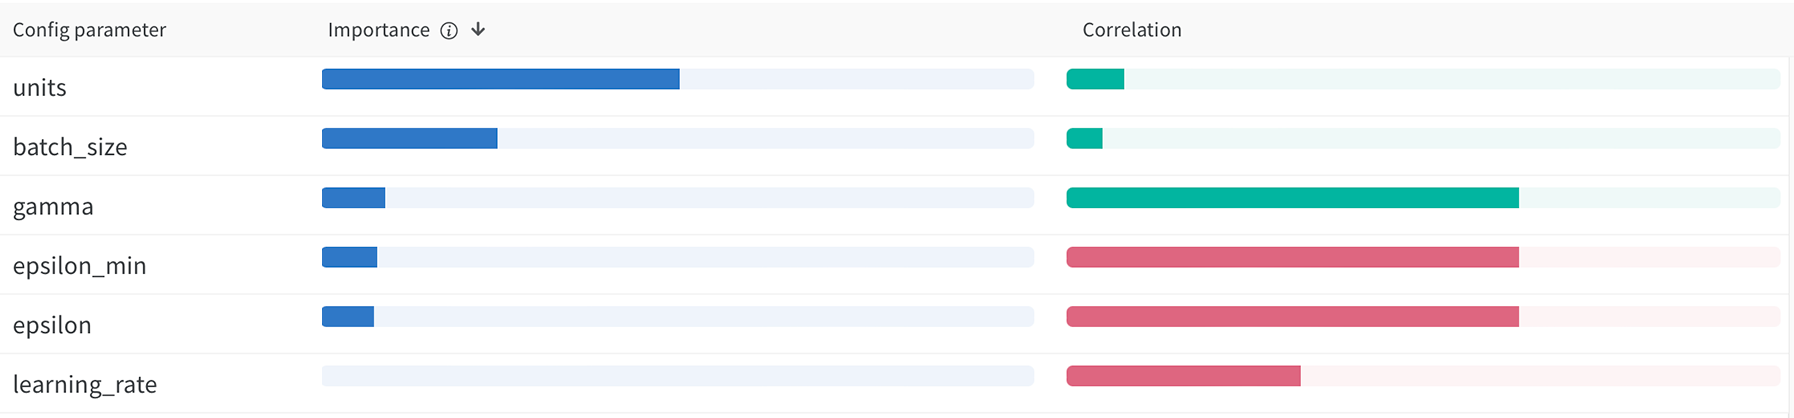
\includegraphics[width=1\textwidth]{selected_walker_importance.png}
 \caption{Importance and correlation analysis of the selected runs. See text for details.}
\label{fig:importance}
\end{figure}

\begin{table}[H]
 \centering
 \caption{Hyperparameters used for the selected experiments explored in this chapter.}
 \label{table:graph_walker}
 \begin{tabular}{|l|l|l|l|l|l|l|}
 \hline
 Hyperparameters & Run 1 & Run 2 & Run 3 & Run 4 & Run 5 & Run 6 \\ \hline
 Batch size & 50 & 12 & 12 & 128 & 32 & 50 \\ \hline
 Epsilon & 0.8 & 0.8 & 0.8 & 0.8 & 0.8 & 0s.3 \\ \hline
 Epsilon minimum & 0.1 & 0.1 & 0.1 & 0.1 & 0.1 & 0.02 \\ \hline
 Gamma & 0.65 & 0.65 & 0.65 & 0.65 & 0.65 & 0.99 \\ \hline
 Learning rate & 0.01 & 0.05 & 0.01 & 0.01 & 0.01 & 0.01 \\ \hline
 Loss & mae & mae & mae & mae & mae & mae \\ \hline
 Units & 128 & 64 & 64 & 64 & 256 & 128 \\ \hline
 \end{tabular}
 \end{table}

The graph \ref{fig:importance} is generated using WandB, it shows the linear \textbf{correlation} between the hyperparameter and the reward obtained, the red lines represent a negative value and the green lines represent positive values, therefore, when the hyperparameter has a higher value, the metric also has higher values and vice versa. Although, correlation alone isn't a very good metric as it does not capture second-hand interactions between parameters.\cite{parameterimportance}
Therefore an importance metric is also calculated using a random forest with the hyperparameters as inputs and the metric as the target output and reports the feature importance values for the random forest.

This analysis shows how the number of units in the neural network impacts the results, coming up as the most important hyperparameter in the testing. The second hyperparameter is batch-size, affecting how much data is fed into the network. Gamma and its high correlation with the episode reward is expected, as a higher gamma values more long-term rewards. The next two hyperparameters, epsilon and epsilon min(minimum), are related, $\epsilon$ is the initial value of exploration while epsilon min is the value of exploration at the end of the episode. The data shows that lower epsilons work better for the tests conducted, it was a common observation, not only in the selected runs, but also along the entire development process. 
In this specific case, higher exploitation works better. The best Run tested, Run 6, $\epsilon$ was set to 0.3 and epsilon minimum to 0.02.
\section{3D Environment}
As mentioned, this scenario, due to time constraints, limited resources and unforeseen challenges in implementing the 2D environment, was not tested using a learning algorithm. Although, this stage was implemented in ROS2 as it was important to have the technology ready for development and testing, not only for walking but to be used by the team to train any suitable tasks.